% !TeX program = xelatex
% Compile from the project root; this increment contains prerequisites only.
\documentclass[12pt,a4paper]{article}
\RequirePackage{array}[=2024-06-01]
% !TeX root = ../2/main.tex
\usepackage[a4paper,margin=25mm,headheight=16pt]{geometry}
\usepackage{amsmath,amssymb}
\usepackage{graphicx}
\usepackage{booktabs}
\usepackage{tabularx}
\usepackage{siunitx}
\usepackage{tikz}
\usepackage{circuitikz}
\usepackage[unicode,hidelinks]{hyperref}
\usepackage{xepersian}
% Only the regular B Nazanin file is installed; synthesize bold explicitly.
\settextfont[Path=C:/Windows/Fonts/,AutoFakeBold=2,AutoFakeSlant=0.2]{B-NAZANIN.TTF}
% B Nazanin lacks U+066A (Arabic percent), required by xepersian's digit setup.
% Arial covers the complete required digit/punctuation set; Persian prose remains B Nazanin.
\setdigitfont[Path=C:/Windows/Fonts/,BoldFont=arialbd.ttf,ItalicFont=ariali.ttf,BoldItalicFont=arialbi.ttf]{arial.ttf}
\setmathdigitfont[Path=C:/Windows/Fonts/,BoldFont=arialbd.ttf,ItalicFont=ariali.ttf,BoldItalicFont=arialbi.ttf]{arial.ttf}
\setlatintextfont{TeX Gyre Termes}
% B Nazanin does not contain the default itemize bullet and dash glyphs.
\renewcommand{\labelitemi}{\(\bullet\)}
\renewcommand{\labelitemii}{\(\circ\)}
\renewcommand{\labelitemiii}{\(\diamond\)}
\setlength{\parindent}{0pt}
\setlength{\parskip}{0.5em}
\linespread{1.25}
\newcommand{\exercise}[1]{\section*{تمرین #1}}
% !TeX root = ../2/main.tex
% Shared title page for every assignment.
% Change only \AssignmentNumber and \AssignmentDate in each main document.

\newcommand{\AssignmentNumber}[1]{\gdef\assignmentnumber{#1}}
\newcommand{\AssignmentDate}[1]{\gdef\assignmentdate{#1}}

\newcommand{\assignmentnumber}{---}
\newcommand{\assignmentdate}{---}

% Stable course metadata
\newcommand{\universityname}{دانشگاه صنعتی امیرکبیر}
\newcommand{\universityalias}{پلی‌تکنیک تهران}
\newcommand{\facultyname}{دانشکده مهندسی کامپیوتر}
\newcommand{\coursename}{طراحی مدارهای مجتمع پرتراکم پیشرفته}
\newcommand{\studentname}{محمد خلیلی اصل}
\newcommand{\instructorname}{دکتر مهدی صدیقی}

\newcommand{\MakeAssignmentCover}{%
  \begin{titlepage}
    \thispagestyle{empty}
    \centering
    \linespread{1}\selectfont

    \vspace*{0mm}
    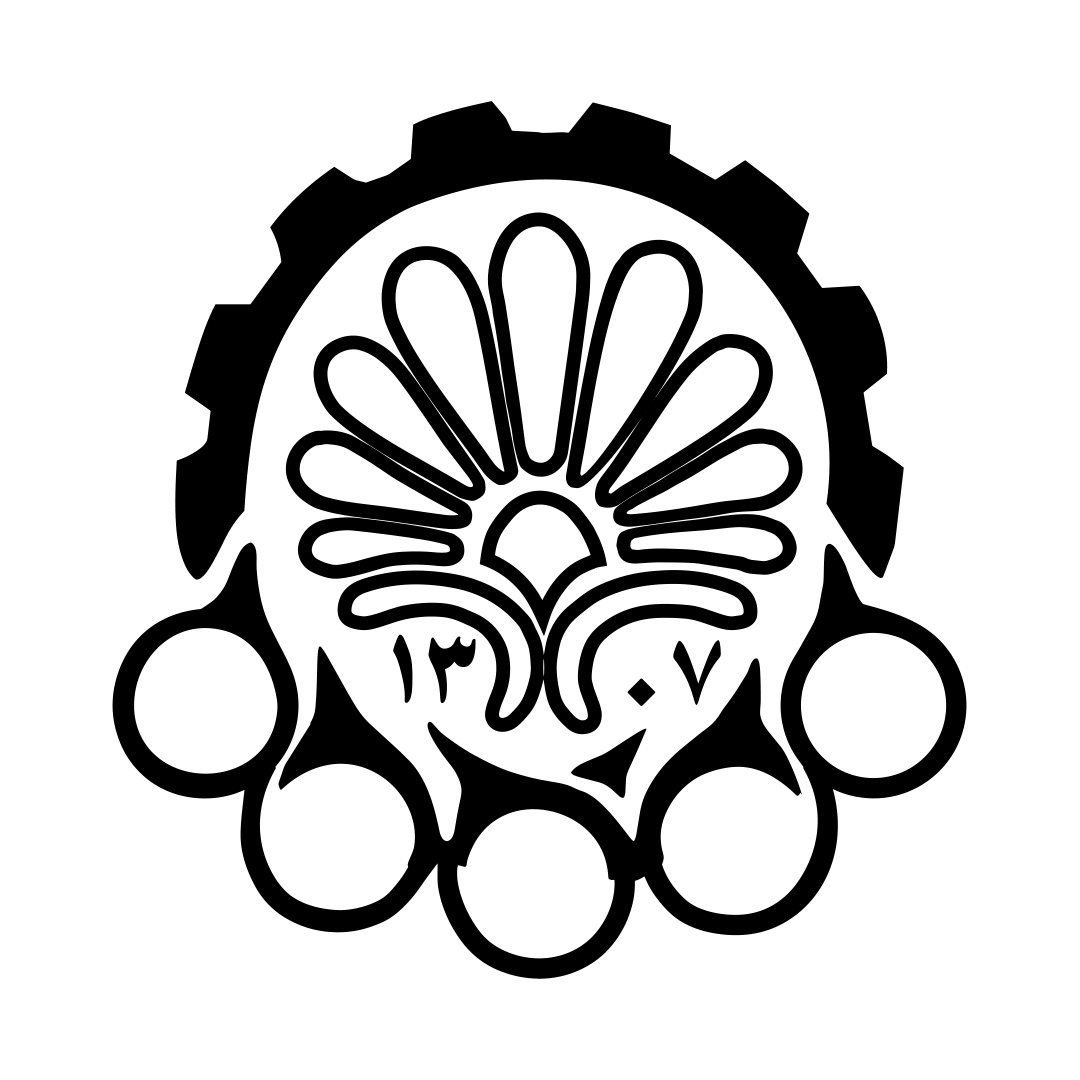
\includegraphics[width=44mm]{assets/aut-logo-black.png}\par
    \vspace{3mm}

    {\Large\bfseries \universityname\par}
    \vspace{1mm}
    {\large (\universityalias)\par}
    \vspace{1mm}
    {\large \facultyname\par}

    \vspace{8mm}
    {\Large\bfseries درس \coursename\par}

    \vspace{12mm}
    {\large عنوان\par}
    \vspace{2mm}
    {\LARGE\bfseries تمرین شماره \assignmentnumber\par}

    \vspace{10mm}
    {\large تهیه‌کننده\par}
    \vspace{2mm}
    {\Large\bfseries \studentname\par}

    \vspace{10mm}
    {\large استاد درس\par}
    \vspace{2mm}
    {\Large\bfseries \instructorname\par}

    \vspace{10mm}
    {\Large \assignmentdate\par}
    \vfill
  \end{titlepage}
  \setcounter{page}{1}%
}


\XeTeXgenerateactualtext=1
\newcommand{\secnum}[1]{\mbox{\beginL#1\endL}}
\setlength{\emergencystretch}{3em}
% Keep SI micro upright in the Latin font; B Nazanin lacks U+00B5.
\AtBeginDocument{\DeclareSIPrefix{\micro}{\text{\lr{µ}}}{-6}}
\widowpenalty=10000
\clubpenalty=10000
\hypersetup{pdftitle={جزوه اول؛ پیش‌نیازهای مدار، ریاضی و منطق دیجیتال}}
\AssignmentNumber{جزوه اول؛ پیش‌نیازهای ضروری}
\AssignmentDate{بخش آغازین؛ نسخه قابل بررسی}
\patchcmd{\MakeAssignmentCover}{تمرین شماره \assignmentnumber}{\assignmentnumber}{}{\errmessage{Cover title replacement failed}}
\begin{document}
\MakeAssignmentCover
\section*{راهنمای مطالعه و دامنه این بخش}
این بخش برای شروع درس بدون گذراندن الکترونیک دیجیتال نوشته شده است.
آشنایی قبلی با قوانین مدار، گیت‌های منطقی یا ریاضیات تحلیل ترانزیستور فرض نمی‌شود.
ابتدا زبان محاسبات، سپس مدار و سرانجام منطق دیجیتال آموزش داده می‌شود.
در خواندن نخست، مثال‌ها را با قلم دوباره محاسبه کنید؛ در پایان هر درس، پاسخ پرسش‌ها
را پیش از خواندن توضیح آن‌ها بنویسید.

این نسخه فقط پیش‌نیازهای جزوه اول است. آموزش کامل فصل ۱ و بخش‌های
\secnum{۲.۱} تا \secnum{۲.۳} کتاب در ادامه تهیه می‌شود.
بنابراین این فایل، جزوه کامل فصل‌های کتاب یا جایگزین دو جزوه بعدی نیست.
نمونه قبلی برای تایید سبک نگارش حفظ شده است؛ مطالب مقدماتی آن در این بخش گسترش یافته‌اند.

مبنای درس، کتاب \lr{Weste} و \lr{Harris} و اسلایدهای محلی است
\cite{weste,intro,mos}. برای مبانی مدار که کتاب درس آن‌ها را پیش‌فرض می‌گیرد،
از \lr{University Physics, Volume 2} استفاده شده است
\cite{current,resistors,kirchhoff,capacitors}.
توضیح‌های ریاضی و مثال‌های با عنوان «مثال آموزشی»، برای این جزوه تنظیم شده‌اند؛
مقادیر آن‌ها مشخصات فناوری یا نتیجه شبیه‌سازی نیستند.

\tableofcontents
\clearpage
% !TeX root = booklet-01.tex
\section{زبان ریاضی لازم برای خواندن مدار}
\label{sec:foundation-math}
فرمول یک رابطه میان کمیت‌هاست. پیش از محاسبه باید بدانیم هر حرف چه کمیتی را
نمایش می‌دهد، واحد آن چیست و رابطه تحت چه فرضی به کار می‌رود.
در این درس، حفظ شکل رابطه بدون شناخت این سه مورد می‌تواند به جواب عددی ظاهراً درست
اما از نظر فیزیکی نامعتبر منجر شود.

\subsection{نماد، زیرنویس، کسر و نسبت}
حرفی مانند \(V\) می‌تواند نماد ولتاژ باشد؛ زیرنویس آن مشخص می‌کند کدام ولتاژ
منظور است. برای مثال، \(V_a\) ولتاژ گره \(a\) و \(V_{ab}\) اختلاف ولتاژ
گره \(a\) نسبت به \(b\) است. زیرنویس، ضرب نیست: \(V_a\) به معنی \(V\times a\) نیست.
نماد \(\Delta\) نیز تغییر کمیت را نشان می‌دهد. برای نمونه، تغییر ولتاژ را
به صورت زیر تعریف می‌کنیم.
\[
 \Delta V=V_{\mathrm{final}}-V_{\mathrm{initial}}.
\]
واژه‌های زیرنویس \(\mathrm{final}\) و \(\mathrm{initial}\) به‌ترتیب حالت نهایی و اولیه‌اند.

در کسر \(a/b\)، صورت \(a\) بر مخرج \(b\) تقسیم می‌شود و باید \(b\ne0\) باشد.
نسبت دو کمیت هم‌واحد، بدون واحد است. مثلاً نسبت \(\qty{6}{\volt}\)
به \(\qty{2}{\volt}\) برابر ۳ است؛ ولی نسبت ولتاژ به جریان واحد دارد
و می‌تواند مقاومت را بیان کند. پس واحدها بخشی از استدلال‌اند.

برای دیدن اثر یک پارامتر، نخست سایر پارامترها را ثابت می‌گیریم.
در رابطه \(y=kx\)، اگر \(k\) ثابت باشد، دو برابر شدن \(x\)، مقدار \(y\) را
دو برابر می‌کند. در \(y=k/x\)، با \(k\) ثابت و \(x\ne0\)، دو برابر شدن
\(x\)، مقدار \(y\) را نصف می‌کند. این نتیجه‌ها وقتی سایر پارامترها نیز
تغییر کنند الزاماً برقرار نیستند.

\subsection{توان و نماد علمی}
توان مثبت، ضرب تکراری است. برای پایه ده و توان سه داریم
\[
 10^3=10\times10\times10=1000.
\]
توان منفی یعنی معکوس توان مثبت. برای همان پایه و توان منفی سه داریم
\[
 10^{-3}=\frac{1}{10^3}=0.001.
\]
قواعد زیر برای پایه مثبت \(a\) و توان‌های مورد استفاده در این جزوه به کار می‌روند:
\begin{equation}\label{eq:foundation-powers}
a^m a^n=a^{m+n},\qquad
\frac{a^m}{a^n}=a^{m-n},\qquad
(a^m)^n=a^{mn}.
\end{equation}
برای نمونه، قانون تفریق توان‌ها در تقسیم می‌دهد
\[
 \frac{10^{-12}}{10^{-9}}=10^{-12-(-9)}=10^{-3}.
\]
دو علامت منفی در تفریق توان‌ها حذف می‌شوند؛ نتیجه \(10^{-21}\) نیست.

در نماد علمی، عدد را به صورت \(b\times10^n\) می‌نویسیم؛ برای عدد مثبت،
معمولاً \(1\le b<10\) است. مثلاً \(0.000024=2.4\times10^{-5}\).
در جمع، باید ابتدا توان‌ها یکسان شوند:
\[
2\times10^{-3}+3\times10^{-4}
=20\times10^{-4}+3\times10^{-4}
=23\times10^{-4}=2.3\times10^{-3}.
\]
قانون جمع توان‌ها در رابطه \eqref{eq:foundation-powers} برای ضرب است؛
به جمع دو عدد تعمیم داده نمی‌شود.

\subsection{واحد و تبدیل پیشوند}
واحدهای مورد استفاده را در جدول \ref{tab:foundation-units} می‌بینیم.
نماد واحد با نماد متغیر تفاوت دارد؛ مثلاً \(C\) متغیر ظرفیت،
ولی \(\mathrm{C}\) نماد واحد بار است.
\begin{table}[ht]
\centering
\caption{کمیت‌ها و واحدهای اصلی این بخش}
\label{tab:foundation-units}
\begin{tabular}{ccc}
\toprule
کمیت & نماد متداول & واحد \lr{SI}\\
\midrule
بار & \(Q\) & \(\mathrm{C}\)\\
جریان & \(I\) & \(\mathrm{A}\)\\
ولتاژ & \(V\) & \(\mathrm{V}\)\\
مقاومت & \(R\) & \(\Omega\)\\
ظرفیت & \(C\) & \(\mathrm{F}\)\\
زمان & \(t\) & \(\mathrm{s}\)\\
انرژی & \(E\) & \(\mathrm{J}\)\\
توان & \(P\) & \(\mathrm{W}\)\\
\bottomrule
\end{tabular}
\end{table}

پیشوندهای \lr{kilo}، \lr{milli}، \lr{micro}، \lr{nano}، \lr{pico} و
\lr{femto} به‌ترتیب ضرایب \(10^3\)، \(10^{-3}\)، \(10^{-6}\)،
\(10^{-9}\)، \(10^{-12}\) و \(10^{-15}\) هستند.
پس \(\qty{2}{\kilo\ohm}=\qty{2000}{\ohm}\) و
\(\qty{20}{\femto\farad}=20\times10^{-15}\,\mathrm{F}\).

\textbf{مثال آموزشی.} برای محاسبه زمان از نسبت بار به جریان، فرض کنید
\(Q=\qty{6}{\pico\coulomb}\) و جریان ثابت \(I=\qty{3}{\milli\ampere}\) باشد:
\begin{align*}
t&=\frac{Q}{I}
=\frac{6\times10^{-12}\,\mathrm{C}}{3\times10^{-3}\,\mathrm{A}}\\
&=2\times10^{-9}\,\mathrm{s}=\qty{2}{\nano\second}.
\end{align*}
چون \(\mathrm{A}=\mathrm{C}/\mathrm{s}\)، واحد کسر برابر ثانیه می‌شود.
این کنترل واحد، مستقل از حساب عددی است و خطای استفاده از \(I/Q\) را آشکار می‌کند.

\subsection{حل معادله با حفظ تساوی}
معادله یعنی دو عبارت مقدار یکسان دارند. برای حفظ این برابری، باید عملی یکسان
روی هر دو طرف انجام دهیم. در \(V=RI\)، برای پیدا کردن جریان و با فرض \(R\ne0\)،
دو طرف را بر \(R\) تقسیم می‌کنیم تا \(I=V/R\) به دست آید.

\textbf{مثال آموزشی.} معادله \(3x+2=11\) را حل کنیم. ابتدا از دو طرف ۲ کم
می‌کنیم و سپس دو طرف را بر ۳ تقسیم می‌کنیم.
\[
 \begin{aligned}
 3x&=9,\\
 x&=3.
 \end{aligned}
\]
جای‌گذاری در معادله اولیه می‌دهد \(3\times3+2=11\).
منظور از «انتقال جمله به طرف دیگر»، همین عمل روی دو طرف است؛ علامت‌ها بی‌دلیل تغییر نمی‌کنند.

توزیع ضرب روی پرانتز یعنی \(a(b+c)=ab+ac\).
بنابراین \(2(x-3)=2x-6\)، نه \(2x-3\).
همچنین \((x-y)^2=x^2-2xy+y^2\)؛ جمله میانی را نباید حذف کرد.
برای تقسیم بر یک عبارت حاوی مجهول، باید صفر نبودن آن را بررسی کنیم؛
تقسیم معادله \(x(x-1)=0\) بر \(x\)، جواب مجاز \(x=0\) را از دست می‌دهد.

\subsection{معادله درجه‌دو و انتخاب ریشه فیزیکی}
وقتی جمله \(x^2\) داریم، ممکن است دو جواب ریاضی وجود داشته باشد.
برای \(ax^2+bx+c=0\) با \(a\ne0\)، تعریف \(D=b^2-4ac\) می‌دهد:
\begin{equation}\label{eq:foundation-quadratic}
x=\frac{-b\pm\sqrt{D}}{2a}.
\end{equation}
در اعداد حقیقی، اگر \(D<0\) باشد جواب حقیقی نداریم؛ اگر \(D=0\)،
دو ریشه بر هم منطبق‌اند و اگر \(D>0\)، دو ریشه متمایز داریم.
نماد \(\pm\) یعنی یک‌بار علامت مثبت و یک‌بار منفی را به کار ببریم.

\textbf{مثال آموزشی بدون واحد.} فرض کنید \(x^2-3x+2=0\) و مسئله شرط
\(0\le x\le1.5\) را نیز داده باشد. در اینجا \(a=1\)، \(b=-3\) و \(c=2\) است:
\[
D=(-3)^2-4(1)(2)=1,\qquad
x=\frac{3\pm1}{2}.
\]
ریشه‌ها ۱ و ۲ هستند. هر دو معادله را ارضا می‌کنند؛ فقط ریشه ۱ در بازه مجاز است.
پس جواب مسئله ۱ است، نه صرفاً ریشه مثبت؛ هر دو ریشه در این مثال مثبت‌اند.
در تحلیل ترانزیستور نیز علاوه بر معادله، باید شرط ناحیه عملکرد و بازه ولتاژها برقرار باشد.

\subsection{خواندن نمودار و معنای شیب}
در نمودار \(y=f(x)\)، محور افقی مقدار \(x\) و محور عمودی مقدار متناظر \(y\)
را نشان می‌دهد. عبارت \(f(x)\) نام یک قانون وابستگی است؛ ضرب \(f\) در \(x\) نیست.
برای دو نقطه، شیب متوسط را تعریف می‌کنیم:
\begin{equation}\label{eq:foundation-slope}
m=\frac{y_2-y_1}{x_2-x_1},\qquad x_2\ne x_1.
\end{equation}
شیب مثبت یعنی در این بازه با افزایش \(x\)، مقدار \(y\) افزایش یافته است؛
شیب منفی یعنی کاهش یافته است. واحد شیب، واحد محور عمودی تقسیم بر واحد محور افقی است.
مثلاً اگر ولتاژ در \(\qty{2}{\nano\second}\) از صفر به \(\qty{1}{\volt}\) برسد،
شیب متوسط \(\qty{0.5}{\volt\per\nano\second}\) است.

مشتق، حد همین نسبت در یک بازه بسیار کوچک است؛ نوشتن \(\mathrm{d}V/\mathrm{d}t\)
یعنی شیب لحظه‌ای نمودار ولتاژ نسبت به زمان، نه تقسیم خود \(V\) بر خود \(t\).
برای خط راست، شیب در همه نقاط ثابت و با شیب متوسط برابر است؛ برای منحنی چنین نیست.
آموزش استخراج مشتق‌ها در محل استفاده از آن‌ها ادامه خواهد یافت.

\subsection{سنجش فهم ریاضی}
\begin{enumerate}
\item \textbf{آیا \(10^{-6}+10^{-6}=10^{-12}\) است؟}
خیر؛ مجموع \(2\times10^{-6}\) است. حاصل‌ضرب آن دو برابر \(10^{-12}\) می‌شود.
\item \textbf{در \(I=V/R\)، با ثابت بودن \(V\)، سه برابر شدن مقاومت چه اثری دارد؟}
جریان به یک‌سوم می‌رسد؛ زیرا مخرج سه برابر شده است.
\item \textbf{آیا هر ریشه‌ای که معادله را ارضا کند جواب مدار است؟}
خیر؛ باید با واحدها، بازه مجاز، اتصال‌ها و فرض‌های مدل نیز سازگار باشد.
\end{enumerate}

% !TeX root = booklet-01.tex
\section{کمیت‌های الکتریکی و خواندن اتصال‌ها}
\label{sec:foundation-circuits}
\subsection{بار، جریان و جهت مرجع}
بار الکتریکی با \(Q\) و واحد \lr{coulomb} نمایش داده می‌شود.
جریان متوسط، بار خالص عبوری از یک مقطع در واحد زمان است \cite{current}:
\begin{equation}\label{eq:foundation-current}
I_{\mathrm{avg}}=\frac{\Delta Q}{\Delta t}.
\end{equation}
برای مثال، عبور \(\qty{6}{\pico\coulomb}\) در \(\qty{2}{\nano\second}\)،
جریان متوسط \(\qty{3}{\milli\ampere}\) می‌دهد.
این رابطه از شکل تغییر جریان در طول بازه اطلاعی نمی‌دهد.
جریان لحظه‌ای با \(i(t)=\mathrm{d}Q/\mathrm{d}t\) بیان می‌شود؛ معنای نرخ تغییر
در بخش \ref{sec:foundation-math} توضیح داده شد.

جهت جریان قراردادی، جهت حرکت بار مثبت است؛ برای حرکت \lr{Electron} در فلز،
جهت حرکت حامل و جریان مخالف‌اند \cite{current}.
در تحلیل، ابتدا یک پیکان مرجع انتخاب می‌کنیم. اگر پاسخ جریان منفی شد،
جهت واقعی مخالف پیکان است؛ منفی شدن لزوماً نشانه اشتباه محاسبه نیست.

\subsection{ولتاژ، مرجع و تفاوت انرژی و توان}
ولتاژ، اختلاف پتانسیل است. تغییر انرژی پتانسیل بار مثبت \(q\) در جابه‌جایی
از نقطه \(b\) به \(a\)، برابر \(\Delta U=q(V_a-V_b)\) است.
بنابراین واحد ولتاژ، انرژی بر بار است:
\(\qty{1}{\volt}=\qty{1}{\joule\per\coulomb}\).
ولتاژ دو نقطه را با ترتیب مشخص تعریف می‌کنیم:
\begin{equation}\label{eq:foundation-voltage}
V_{ab}=V_a-V_b,\qquad V_{ba}=-V_{ab}.
\end{equation}
اگر \(V_a=\qty{1}{\volt}\) و \(V_b=\qty{0.4}{\volt}\)،
داریم \(V_{ab}=\qty{0.6}{\volt}\).
ولتاژ گره به‌تنهایی، همیشه نسبت به مرجعی مثل \lr{Ground} معنا دارد.
تغییر مرجع مشترک، اختلاف ولتاژ واقعی دو گره را تغییر نمی‌دهد.

انرژی مقدار کار قابل مبادله است؛ توان، نرخ مبادله انرژی است.
اگر جریان \(i\) وارد سر مثبت ولتاژ \(v\) یک جزء شود، توان جذب‌شده آن جزء
\(p=vi\) است. حاصل مثبت یعنی جذب و حاصل منفی یعنی تحویل انرژی به مدار.
این رابطه و کاربرد \(P=VI\) در تحلیل توان مدار با بخش \secnum{۱.۹} کتاب مرتبط‌اند
\cite{weste}. مثلاً یک مقاومت با ولتاژ \(\qty{1}{\volt}\) و جریان
\(\qty{1}{\milli\ampere}\)، توان \(\qty{1}{\milli\watt}\) جذب می‌کند؛
اگر این وضع \(\qty{2}{\milli\second}\) ثابت بماند، انرژی جذب‌شده
\(E=Pt=\qty{2}{\micro\joule}\) است. انرژی و توان هم‌واحد نیستند.

\subsection{گره، شاخه، مدار باز و اتصال کوتاه}
\lr{Node} مجموعه نقاطی است که با سیم ایدئال مستقیم متصل و هم‌پتانسیل‌اند.
وجود یک قطعه میان دو نقطه، معمولاً آن‌ها را به دو گره متفاوت تبدیل می‌کند.
\lr{Branch} یک مسیر میان دو گره است که جریان آن را در تحلیل مشخص می‌کنیم.
\lr{Ground} گره مرجع با ولتاژ صفر است؛ الزامی ندارد به زمین فیزیکی متصل باشد.

در نقشه‌های کتاب، اتصال به‌شکل \lr{T} متصل است؛ برای تقاطع دو سیم،
وجود نقطه، اتصال را مشخص می‌کند \cite[بخش \secnum{۱.۴.۲}]{weste}.
ظاهر نزدیک یا دور دو قطعه معیار هم‌گره بودن نیست؛ مسیر سیم را باید دنبال کرد.

در مدل \lr{Open Circuit}، جریان مسیر باز صفر است، ولی اختلاف ولتاژ دو سر آن
می‌تواند غیرصفر باشد. در مدل \lr{Short Circuit}، اختلاف ولتاژ صفر است؛
جریان را بقیه مدار تعیین می‌کند. اتصال کوتاه مستقیم دو سر منبع ولتاژ ایدئال
غیرصفر، مدلی ناسازگار ایجاد می‌کند؛ برای محاسبه جریان واقعی باید مقاومت‌ها و
محدودیت‌های منبع را در نظر گرفت.

\section{قوانین مدار و روش تحلیل}
\subsection{مقاومت و \lr{Ohm's Law}}
برای مقاومت خطی مثبت \(R\)، با ورود جریان مرجع به سر مثبت ولتاژ، داریم
\cite{resistors}:
\begin{equation}\label{eq:foundation-ohm}
v=Ri,\qquad i=\frac{v}{R}.
\end{equation}
مقاومت بزرگ‌تر در ولتاژ ثابت، جریان کمتری می‌دهد.
اگر جریان محاسبه‌شده منفی شود، جهت مرجع برعکس جریان واقعی بوده است.
از \(p=vi\) و رابطه \eqref{eq:foundation-ohm} نتیجه می‌گیریم
\(p=Ri^2=v^2/R\ge0\). پس مقاومت مثبت در این مدل انرژی تولید نمی‌کند.
ترانزیستور را نباید در تمام ناحیه‌های عملکرد، یک مقاومت ثابت فرض کرد؛
رابطه جریان آن در ادامه جزوه استخراج خواهد شد.

\subsection{قانون گره: \lr{KCL}}
در مدل مدار متمرکز، با حساب‌کردن جریان تمام شاخه‌ها از جمله شاخه‌های خازنی،
مجموع جریان‌های ورودی به گره با مجموع جریان‌های خروجی برابر است
\cite{kirchhoff}. این قانون با نام \lr{Kirchhoff's Current Law (KCL)} شناخته می‌شود:
\begin{equation}\label{eq:foundation-kcl}
\sum I_{\mathrm{in}}=\sum I_{\mathrm{out}}.
\end{equation}
نماد \(\sum\) یعنی جمع‌کردن همه جمله‌های مربوط.
مثلاً اگر \(\qty{3}{\milli\ampere}\) وارد گره و
\(\qty{1}{\milli\ampere}\) از یک شاخه خارج شود، جریان خروجی شاخه دیگر
\(\qty{2}{\milli\ampere}\) است. اگر خروجی به خازن متصل باشد، نباید
جریان شارژ آن را از معادله حذف کنیم.

\subsection{قانون حلقه: \lr{KVL}}
در تحلیل مدار متمرکز و با صرف‌نظر از القای مغناطیسی مدل‌نشده، جمع جبری تغییرات
ولتاژ در پیمودن یک مسیر بسته صفر است \cite{kirchhoff}.
این \lr{Kirchhoff's Voltage Law (KVL)} است:
\begin{equation}\label{eq:foundation-kvl}
\sum_{\mathrm{loop}}\Delta V=0.
\end{equation}
در عبور از منبع از پایانه منفی به مثبت، افزایش ولتاژ داریم؛ در عبور از مقاومت
در جهت جریان، افت \(IR\) داریم. مثلاً منبع \(V_s\) و دو مقاومت سری می‌دهند
\(V_s-IR_1-IR_2=0\). از اینجا
\(I=V_s/(R_1+R_2)\) به دست می‌آید. جهت پیمودن حلقه دلخواه است؛
باید علامت‌ها با همان انتخاب سازگار بمانند.

\subsection{اتصال \lr{Series} و \lr{Parallel} را از گره‌ها بشناسیم}
دو مقاومت وقتی سری‌اند که گره مشترکشان شاخه دیگری نداشته باشد؛ جریان یکسانی از
هر دو می‌گذرد. از جمع افت ولتاژها، \(R_{\mathrm{eq}}=R_1+R_2\) نتیجه می‌شود.
وقتی دو مقاومت دقیقاً میان دو گره یکسان باشند، موازی‌اند و ولتاژ یکسانی دارند.
با جمع جریان‌ها طبق \lr{KCL} به دست می‌آید \cite{resistors}:
\begin{align}
I&=\frac{V}{R_1}+\frac{V}{R_2}
=V\left(\frac{1}{R_1}+\frac{1}{R_2}\right),\notag\\
\frac{1}{R_{\mathrm{eq}}}&=\frac{1}{R_1}+\frac{1}{R_2},
\qquad R_{\mathrm{eq}}=\frac{R_1R_2}{R_1+R_2}.
\label{eq:foundation-parallel}
\end{align}
برای دو مقاومت مثبت، مقاومت معادل موازی از هر دو کمتر است؛ این یک کنترل مفید برای جواب است.
مثلاً دو مقاومت \(\qty{2}{\kilo\ohm}\) و \(\qty{3}{\kilo\ohm}\)،
در سری \(\qty{5}{\kilo\ohm}\) و در موازی \(\qty{1.2}{\kilo\ohm}\) می‌دهند.

\subsection{مثال کامل: استخراج ولتاژ یک گره}
در شکل \ref{fig:foundation-divider}، منبع ایدئال \(V_s\) و دو مقاومت مثبت داریم.
خروجی بار رسانشی ندارد. شکل برای همین جزوه رسم شده است.
\begin{figure}[ht]
\centering
\begin{latin}
\begin{circuitikz}[american]
\draw (0,0) node[ground] {} to[V,invert,l=$V_s$] (0,3)
 to[R,l=$R_1$] (3,3) to[R,l=$R_2$] (3,0) -- (0,0);
\draw (3,3) to[short,*-o] (4.7,3) node[right] {$V_x$};
\end{circuitikz}
\end{latin}
\caption{مدار آموزشی تقسیم ولتاژ؛ خروجی از گره مشترک دو مقاومت گرفته می‌شود.}
\label{fig:foundation-divider}
\end{figure}
جریان \(R_1\) را از منبع به گره \(x\) و جریان \(R_2\) را از گره به زمین
انتخاب می‌کنیم. ولتاژهای دو سر مقاومت‌ها به‌ترتیب \(V_s-V_x\) و \(V_x-0\) هستند.
با استفاده از \lr{Ohm's Law} و سپس \lr{KCL}:
\begin{align}
\frac{V_s-V_x}{R_1}&=\frac{V_x}{R_2},\notag\\
R_2(V_s-V_x)&=R_1V_x,\notag\\
R_2V_s&=(R_1+R_2)V_x,\notag\\
V_x&=V_s\frac{R_2}{R_1+R_2}.
\label{eq:foundation-divider}
\end{align}
در سطر دوم دو طرف را در \(R_1R_2\) ضرب کردیم؛ سپس پرانتز را باز و جمله‌های
حاوی \(V_x\) را یک طرف جمع کردیم. با \(V_s=\qty{1}{\volt}\)،
\(R_1=\qty{2}{\kilo\ohm}\) و \(R_2=\qty{3}{\kilo\ohm}\)،
داریم \(V_x=\qty{0.6}{\volt}\).
جریان هر دو مقاومت \(\qty{0.2}{\milli\ampere}\) و افت‌ها
\(\qty{0.4}{\volt}\) و \(\qty{0.6}{\volt}\) هستند؛ جمع افت‌ها با منبع برابر است.

\textbf{کنترل حدی و فرض بار.} با میل \(R_2\) به صفر، خروجی به صفر و با
بسیار بزرگ شدن آن نسبت به \(R_1\)، خروجی به \(V_s\) نزدیک می‌شود.
اگر بار مقاومتی \(R_L\) از خروجی به زمین وصل شود، در رابطه
\eqref{eq:foundation-divider} باید \(R_2\) را با \(R_2\parallel R_L\) جایگزین کرد؛
زیرا دیگر جریان \(R_1\) فقط از \(R_2\) نمی‌گذرد. نماد \(\parallel\) اتصال موازی را نشان می‌دهد.

\section{خازن، شارژ و مفهوم زمان}
\label{sec:foundation-capacitor}
\subsection{خازن چه چیزی را ذخیره می‌کند؟}
خازن از دو رسانا با ماده عایق میان آن‌ها ساخته می‌شود.
در مدل دوصفحه‌ای ایدئال، بارهای صفحات \(+Q\) و \(-Q\) هستند؛
مجموع بار دو صفحه می‌تواند صفر باشد، درحالی‌که انرژی در میدان ذخیره شده است
\cite{capacitors}. پس عبارت «بار خازن» معمولاً به بار علامت‌دار یک صفحه
یا اندازه بار صفحات اشاره دارد، نه مجموع آن دو.

اگر ظرفیت ثابت \(C\) باشد و \(v\) را ولتاژ صفحه اول نسبت به دوم بگیریم،
بار صفحه اول برابر است با:
\begin{equation}\label{eq:foundation-qcv}
Q=Cv,\qquad C=\frac{Q}{v}\quad(v\ne0).
\end{equation}
واحد ظرفیت \lr{farad} است و \(\mathrm{F}=\mathrm{C}/\mathrm{V}\).
مثلاً در خازن \(\qty{20}{\femto\farad}\)، ولتاژ \(\qty{1}{\volt}\)
با بار \(\qty{20}{\femto\coulomb}\) روی صفحه مثبت همراه است.
ظرفیت بزرگ‌تر در ولتاژ یکسان، بار بیشتری لازم دارد.

\subsection{از تغییر بار به تغییر ولتاژ}
برای ظرفیت ثابت، از رابطه \eqref{eq:foundation-qcv} داریم
\(\Delta Q=C\Delta v\). تقسیم دو طرف بر \(\Delta t\) و استفاده از تعریف
جریان متوسط می‌دهد:
\begin{equation}\label{eq:foundation-cap-current}
I_{\mathrm{avg}}=C\frac{\Delta v}{\Delta t},
\qquad i(t)=C\frac{\mathrm{d}v}{\mathrm{d}t}.
\end{equation}
در این قرارداد، جریان وارد صفحه‌ای می‌شود که ولتاژ مثبت برای آن تعریف شده است.
جریان مثبت بار آن صفحه و ولتاژ آن را افزایش می‌دهد؛ جریان منفی کاهش می‌دهد.
رابطه دوم شکل لحظه‌ای همان رابطه اول است. این ارتباط مبنای توضیح زمان تغییر خروجی
در کتاب و اسلاید است \cite[بخش \secnum{۱.۹}]{weste}\cite[اسلاید ۸]{mos}.
برای ظرفیت وابسته به ولتاژ، باید به رابطه عمومی \(i=\mathrm{d}Q/\mathrm{d}t\)
برگردیم؛ ثابت گرفتن \(C\) یک فرض مدل است.

\textbf{مثال آموزشی.} فرض کنیم جریان خالص ثابت \(I=\qty{10}{\micro\ampere}\)
به خازن \(C=\qty{20}{\femto\farad}\) وارد شود و ولتاژ آن از
\(\qty{0.2}{\volt}\) به \(\qty{0.8}{\volt}\) برسد. تغییر ولتاژ
\(\Delta v=\qty{0.6}{\volt}\) است. پس:
\begin{align}
\Delta t&=\frac{C\Delta v}{I}
=\frac{(20\times10^{-15}\,\mathrm{F})(0.6\,\mathrm{V})}
{10\times10^{-6}\,\mathrm{A}}\notag\\
&=1.2\times10^{-9}\,\mathrm{s}=\qty{1.2}{\nano\second}.
\label{eq:foundation-charge-time}
\end{align}
واحد \(\mathrm{F}\,\mathrm{V}/\mathrm{A}\) برابر ثانیه است.
در این مدل، دو برابر شدن ظرفیت، زمان را دو برابر و دو برابر شدن جریان، زمان را نصف می‌کند.
این نتیجه برای جریان ثابت است؛ جریان ترانزیستور واقعی عموماً طی تغییر ولتاژ ثابت نیست.

\subsection{حالت ماندگار، گذرا و پاسخ ساده \lr{RC}}
در حالت ماندگار \lr{DC}، ولتاژ خازن ثابت است؛ بنابراین در مدل ایدئال
\(\mathrm{d}v/\mathrm{d}t=0\) و جریان آن صفر می‌شود. این به معنی صفر بودن ولتاژ آن نیست.
در حالت گذرا، بار و ولتاژ تغییر می‌کنند. اختلاف ولتاژ خازن در حضور جریان محدود
نمی‌تواند ناگهان جهش کند؛ چون جهش نیازمند انتقال بار محدود در زمان صفر است.

برای درک تفاوت با جریان ثابت، خازنی را در نظر بگیرید که از منبع ثابت \(V_s\)
از طریق مقاومت \(R\) شارژ می‌شود؛ بار دیگری وجود ندارد و \(v(0)=0\).
با افزایش ولتاژ خازن، اختلاف ولتاژ مقاومت کم می‌شود؛ در نتیجه جریان
\(i=(V_s-v)/R\) کاهش می‌یابد. پس نمودار ولتاژ خط راست نیست.
از \lr{KCL} و رابطه \eqref{eq:foundation-cap-current} به دست می‌آید:
\begin{equation}\label{eq:foundation-rc-ode}
C\frac{\mathrm{d}v}{\mathrm{d}t}=\frac{V_s-v}{R}.
\end{equation}
جواب زیر فعلاً برای تفسیر معرفی می‌شود؛ می‌توان درستی آن را با مشتق‌گیری کنترل کرد:
\begin{equation}\label{eq:foundation-rc}
v(t)=V_s\left(1-e^{-t/(RC)}\right),\qquad t\ge0.
\end{equation}
عدد \(e\approx2.718\) پایه تابع نمایی است. برای عدد بی‌بعد مثبت \(x\)،
\(e^{-x}=1/e^x\)؛ با بزرگ شدن \(x\)، این مقدار به صفر نزدیک می‌شود.
حاصل \(RC\) واحد زمان دارد و آن را ثابت زمانی \(\tau=RC\) می‌نامیم.
در \(t=0\)، جواب صفر است؛ در \(t=\tau\)، مقدار ولتاژ تقریباً
\(0.632V_s\) و با زیاد شدن زمان، حد آن \(V_s\) است.
در مدل ایدئال نمایی، رسیدن دقیق به حد در زمان محدود رخ نمی‌دهد.

شکل \ref{fig:foundation-rc} همین پاسخ را بدون وابستگی به مقیاس یک فناوری
نشان می‌دهد. محور افقی زمان تقسیم بر ثابت زمانی و محور عمودی ولتاژ تقسیم بر
ولتاژ منبع است؛ هر دو نسبت بدون واحدند. کم‌شدن شیب یعنی کاهش جریان شارژ.
\begin{figure}[ht]
\centering
\begin{latin}
\begin{tikzpicture}[x=1.6cm,y=2.6cm]
\draw[->] (0,0) -- (3.6,0) node[right] {$t/\tau$};
\draw[->] (0,0) -- (0,1.25) node[above] {$v/V_s$};
\draw[dashed] (0,1) -- (3.3,1);
\node[left] at (0,1) {\rl{۱}};
\node[below left] at (0,0) {\rl{۰}};
\foreach \x/\ticklabel in {1/۱,2/۲,3/۳} {\draw (\x,0.025) -- (\x,-0.025) node[below] {\rl{\ticklabel}};}
\draw[thick,domain=0:3.3,samples=70] plot (\x,{1-exp(-\x)});
\draw[dotted] (1,0) -- (1,{1-exp(-1)}) -- (0,{1-exp(-1)});
\fill (1,{1-exp(-1)}) circle (1.4pt);
% Match the shared digit font for the Persian decimal separator.
\node[left] at (0,{1-exp(-1)}) {\fontspec[Path=C:/Windows/Fonts/]{arial.ttf}\mbox{\beginL۰٫۶۳۲\endL}};
\end{tikzpicture}
\end{latin}
\caption{نمودار تحلیلی پاسخ \lr{RC} رابطه \eqref{eq:foundation-rc}؛
این شکل از خود رابطه رسم شده است و نتیجه شبیه‌سازی \lr{SPICE} نیست.}
\label{fig:foundation-rc}
\end{figure}

برای دیدن سازگاری جواب با معادله، پاسخ و مشتق آن را کنار هم می‌نویسیم.
\[
 \begin{aligned}
 v&=V_s(1-e^{-t/\tau}),\\
 \frac{\mathrm{d}v}{\mathrm{d}t}&=\frac{V_s}{\tau}e^{-t/\tau}.
 \end{aligned}
\]
پس دو طرف رابطه \eqref{eq:foundation-rc-ode} برابر
\((V_s/R)e^{-t/\tau}\) می‌شوند. قاعده مشتق نمایی در اینجا معرفی شده است؛
استخراج تفصیلی قواعد مشتق در محل نیاز بعدی آموزش داده می‌شود.

\subsection{پرسش‌های مدار با پاسخ}
\begin{enumerate}
\item \textbf{در تقسیم ولتاژ با دو مقاومت مساوی و خروجی بی‌بار، خروجی چقدر است؟}
نصف منبع؛ زیرا \(R/(R+R)=1/2\). این حکم برای خروجی بارگذاری‌شده الزاماً برقرار نیست.
\item \textbf{اگر ولتاژ یک خازن ایدئال ثابت باشد، چه چیزی درباره جریان می‌دانیم؟}
جریان خازن صفر است، ولی شاخه‌های دیگر مدار می‌توانند جریان غیرصفر داشته باشند.
\item \textbf{چرا مدل جریان ثابت و مدل شارژ مقاومتی دو نمودار متفاوت می‌دهند؟}
در اولی شیب \(I/C\) ثابت است؛ در دومی جریان با افزایش ولتاژ خازن کاهش می‌یابد.
\item \textbf{اگر جواب جریان یک مقاومت منفی شد، چه کنیم؟}
ابتدا جهت مرجع و قطب‌های ولتاژ را کنترل کنیم؛ اگر معادله‌ها سازگار باشند،
علامت منفی فقط جهت مخالف جریان واقعی را نشان می‌دهد.
\end{enumerate}

% !TeX root = booklet-01.tex
\section{از ولتاژ فیزیکی به منطق دیجیتال}
\subsection{چرا مقدار منطقی با ولتاژ یکی نیست؟}
سیگنال فیزیکی مدار، ولتاژ یا جریان است؛ مدل دیجیتال بخشی از این رفتار را با
مقادیر گسسته صفر و یک توصیف می‌کند. سیگنال \lr{Analog} می‌تواند در یک بازه
مقادیر پیوسته داشته باشد؛ در توصیف \lr{Digital}، بازه‌هایی از ولتاژ به مقدارهای
منطقی نگاشت می‌شوند. خود ولتاژ واقعی مدار دیجیتال نیز هنگام تغییر پیوسته است.
در قرارداد این درس، ولتاژ نزدیک \lr{Ground} نماینده صفر و نزدیک
\(V_{\mathrm{DD}}\) نماینده یک است \cite[بخش \secnum{۱.۳}]{weste}.
نماد \(V_{\mathrm{DD}}\) نام ریل تغذیه مثبت است، نه یک مقدار ثابت همگانی.

\textbf{مثال آموزشی با مرزهای فرضی.} فرض کنید در مداری با تغذیه
\(\qty{1}{\volt}\)، ورودی از صفر تا \(\qty{0.3}{\volt}\) صفر معتبر و
از \(\qty{0.7}{\volt}\) تا تغذیه یک معتبر تعریف شود.
ولتاژ \(\qty{0.2}{\volt}\) صفر معتبر است، هرچند صفر ولت نیست؛
\(\qty{0.8}{\volt}\) یک معتبر و \(\qty{0.5}{\volt}\) در بازه نامعین است.
این مرزها صرفاً برای آموزش‌اند و مشخصات یک فناوری واقعی را بیان نمی‌کنند.
سطح‌های معتبر و \NotesTopic{sec:noise-margin}{\lr{Noise Margin}} از
مشخصه انتقال مدار استخراج می‌شوند.

\subsection{بیت، بردار و شمارش حالت‌ها}
یک \lr{Bit} یک مقدار دودویی دارد. دو بیت مستقل چهار ترکیب و \(n\) بیت مستقل
\(2^n\) ترکیب دارند؛ هر بیت تعداد حالت‌ها را دو برابر می‌کند.
برای سه ورودی، بنابراین هشت سطر در جدول کامل نیاز داریم.
برای آشنایی با نمایش عددی، سه بیت \(b_2,b_1,b_0\) در نمایش بدون علامت، عدد
\(4b_2+2b_1+b_0\) را نمایش می‌دهند. مثلاً بیت‌های ۱، ۰، ۱ مقدار ۵ دارند.
اما هر بردار منطقی الزاماً عدد نیست؛ می‌تواند سه سیگنال کنترل مستقل باشد.

\section{گیت‌های پایه و \lr{Truth Table}}
\subsection{تعریف عملگرها و ترتیب محاسبه}
\lr{Truth Table} خروجی را برای تمام ترکیب‌های مجاز ورودی می‌نویسد.
در این بخش ورودی‌ها فقط صفر یا یک هستند.
\lr{NOT} مقدار را معکوس می‌کند؛ آن را با خط بالای متغیر می‌نویسیم:
\(\overline{0}=1\) و \(\overline{1}=0\).
این خط علامت منفی عددی نیست.

عملگر \lr{AND} فقط وقتی یک است که همه ورودی‌ها یک باشند؛ نماد آن
\(A\cdot B\) یا \(AB\) است.
عملگر \lr{OR} وقتی یک است که دست‌کم یک ورودی یک باشد؛ نماد آن \(A+B\) است.
در اینجا \(+\) جمع معمولی نیست: \(1+1=1\) در جبر منطقی.
\lr{XOR} برای دو ورودی وقتی یک است که ورودی‌ها متفاوت باشند و با
\(A\oplus B\) نمایش داده می‌شود. \lr{NAND}، \lr{NOR} و \lr{XNOR}
به‌ترتیب مکمل \lr{AND}، \lr{OR} و \lr{XOR} هستند.
این تعریف‌ها زمینه خواندن گیت‌های بخش \secnum{۱.۴} کتاب را فراهم می‌کنند \cite{weste}.

جدول \ref{tab:foundation-gates} تمام حالت‌های دو ورودی را نشان می‌دهد.
برای جلوگیری از ابهام، در روابط ترکیبی از پرانتز استفاده می‌کنیم؛
در قرارداد متعارف، \lr{NOT} پیش از \lr{AND} و سپس \lr{OR} محاسبه می‌شود.
\begin{table}[ht]
\centering
\caption{جدول گیت‌های دوورودی؛ همه مدخل‌ها مقدار منطقی بدون واحد هستند.}
\label{tab:foundation-gates}
\begin{tabular}{cccccccc}
\toprule
\(A\)&\(B\)&\lr{AND}&\lr{OR}&\lr{XOR}&\lr{NAND}&\lr{NOR}&\lr{XNOR}\\
\midrule
۰&۰&۰&۰&۰&۱&۱&۱\\
۰&۱&۰&۱&۱&۱&۰&۰\\
۱&۰&۰&۱&۱&۱&۰&۰\\
۱&۱&۱&۱&۰&۰&۰&۱\\
\bottomrule
\end{tabular}
\end{table}
برای مثال، در سطر آخر، \lr{OR} یک ولی \lr{XOR} صفر است؛
پس «یا»ی \lr{OR} حالت هم‌زمان یک بودن هر دو ورودی را حذف نمی‌کند.

\subsection{مثال مرحله‌ای و ساخت جدول از عبارت}
برای عبارت \(Y=\overline{AB+C}\)، ابتدا \(AB\)، سپس \(AB+C\) و در پایان
مکمل کل عبارت را محاسبه می‌کنیم. با \(A=1\)، \(B=0\) و \(C=1\)،
داریم \(AB=0\)، سپس \(0+1=1\) و در نتیجه \(Y=0\).
خط مکمل فقط روی \(C\) نیست؛ محل و طول آن جزئی از تعریف تابع است.

برای ساخت جدول کامل، هر هشت ترکیب ورودی را می‌نویسیم و ستون میانی \(AB\)
را پیش از \(Y\) محاسبه می‌کنیم. راه فشرده‌تر برای فهم نتیجه این است:
اگر \(C=1\)، خروجی در همه حالت‌ها صفر است؛ اگر \(C=0\)،
داریم \(Y=\overline{AB}\). پس خروجی فقط در سه حالت
\((A,B,C)=(0,0,0),(0,1,0),(1,0,0)\) یک است.
این نتیجه با تعریف \lr{NAND} در جدول \ref{tab:foundation-gates} قابل کنترل است.

\subsection{از جدول به عبارت منطقی}
اگر خروجی تابعی فقط برای دو حالت \((A,B)=(0,1)\) و \((1,0)\) یک باشد،
برای حالت اول عبارت \(\overline{A}B\) و برای حالت دوم \(A\overline{B}\) را می‌نویسیم.
هر عبارت فقط همان حالت خود را تشخیص می‌دهد. سپس آن‌ها را با \lr{OR} ترکیب می‌کنیم:
\begin{equation}\label{eq:foundation-xor}
Y=\overline{A}B+A\overline{B}=A\oplus B.
\end{equation}
بنابراین جدول، عبارت و شبکه گیت‌ها سه نمایش مرتبط از یک تابع‌اند.
برای تعداد ورودی زیاد، روش‌های ساده‌سازی کارآمدتری وجود دارد؛
در این بخش هدف فهم نگاشت میان این نمایش‌هاست.

\section{جبر منطقی و اتصال \lr{Switch}ها}
\subsection{قانون‌های موردنیاز و کنترل آن‌ها}
برای متغیر دودویی \(A\)، روابط زیر از بررسی دو مقدار صفر و یک به دست می‌آیند:
\begin{align}
A+0&=A,& A\cdot1&=A,& A+1&=1,& A\cdot0&=0,\notag\\
A+A&=A,& AA&=A,& A+\overline{A}&=1,& A\overline{A}&=0.
\label{eq:foundation-identities}
\end{align}
مثلاً \(A+A=A\) نشان می‌دهد نباید جمع منطقی را مانند جمع عددی
به \(2A\) تبدیل کنیم.
دو قانون پرکاربرد دیگر، توزیع \(A(B+C)=AB+AC\) و جذب
\(A+AB=A\) هستند. برای جذب، اگر \(A=1\)، خروجی در هر صورت یک است؛
اگر \(A=0\)، هر دو جمله صفرند. پس دو طرف در همه حالت‌ها برابرند.

\lr{De Morgan's Laws} می‌گویند مکمل \lr{AND} برابر \lr{OR} مکمل‌ها و
مکمل \lr{OR} برابر \lr{AND} مکمل‌هاست \cite[بخش \secnum{۱.۴}]{weste}:
\begin{equation}\label{eq:foundation-demorgan}
\overline{AB}=\overline{A}+\overline{B},\qquad
\overline{A+B}=\overline{A}\,\overline{B}.
\end{equation}
برای رابطه اول، خروجی فقط وقتی صفر است که هر دو ورودی یک باشند؛
در غیر این صورت حداقل یک مکمل، یک است. این استدلال تمام چهار حالت را پوشش می‌دهد.
پس هنگام بردن مکمل داخل پرانتز، هم متغیرها مکمل می‌شوند و هم عملگر عوض می‌شود.

\textbf{مثال آموزشی.} با جذب داریم
\[
 F=A+\overline{A}B=(A+\overline{A})(A+B)=A+B.
\]
در این تبدیل از قانون توزیع دیگر جبر منطقی،
\(X+YZ=(X+Y)(X+Z)\)، استفاده شده است.
می‌توان بدون حفظ قانون نیز بررسی کرد: اگر \(A=1\)، هر دو طرف یک‌اند؛
اگر \(A=0\)، هر دو طرف برابر \(B\) هستند.

\subsection{چرا اتصال سری با \lr{AND} ارتباط دارد؟}
فعلاً \lr{Switch} ایدئالی را فرض می‌کنیم که با کنترل یک بسته می‌شود.
در دو \lr{Switch} سری، مسیر تنها وقتی بسته است که هر دو بسته باشند؛
پس شرط هدایت \(AB\) است. در دو \lr{Switch} موازی، بسته بودن یکی کافی است؛
پس شرط هدایت \(A+B\) است \cite[اسلاید ۲۲]{intro}.
این‌ها شرط هدایت مسیرند، نه الزاماً مقدار منطقی ولتاژ خروجی.
اگر شبکه مسیر خروجی به زمین را بسازد، برقرار شدن شرط هدایت می‌تواند خروجی را صفر کند.

در اتصال متعارف ریل‌به‌ریل، \lr{nMOS} با ورودی یک و \lr{pMOS} با ورودی صفر
هدایت می‌کند \cite[بخش \secnum{۱.۳}]{weste}\cite[اسلاید ۲۱]{intro}.
بنابراین برای \lr{pMOS} با کنترل \(A\)، شرط هدایت \(\overline{A}\) است.
این عبارت یک مدل مقدماتی برای اتصال مشخص است؛ شرط عمومی روشن شدن به اختلاف ولتاژ
\lr{Gate} و \lr{Source} و آستانه نیاز دارد.

\textbf{پل به تحلیل گیت.} دو \lr{nMOS} سری با کنترل \(A\) و \(B\)،
خروجی را وقتی \(AB=1\) به زمین وصل می‌کنند. برای داشتن گیت معتبر،
شبکه بالایی باید در بقیه حالت‌ها خروجی را به تغذیه برساند و در حالت اول قطع باشد.
با دو \lr{pMOS} موازی، شرط هدایت بالا
\(\overline{A}+\overline{B}=\overline{AB}\) است؛
پس تابع خروجی \(Y=\overline{AB}\)، یعنی \lr{NAND} خواهد بود.
طراحی شماتیک و تحلیل تفصیلی آن در بخش فصل اول دنبال می‌شود.

\section{مدارهای \lr{Combinational} و \lr{Sequential}}
\subsection{وابستگی به ورودی و وابستگی به گذشته}
در مدار \lr{Combinational}، پس از گذشت زمان لازم برای پایدار شدن،
خروجی از ورودی‌های همان زمان تعیین می‌شود. گیت‌های پایه و \lr{Multiplexer}
از نمونه‌های آن‌اند. وجود تاخیر فیزیکی، مدار را به‌خودی‌خود \lr{Sequential} نمی‌کند.

در مدار \lr{Sequential}، خروجی یا حالت بعدی علاوه بر ورودی، به حالت ذخیره‌شده
قبلی وابسته است. مثلاً شمارنده با ورودی کنترلی یکسان می‌تواند بسته به عدد قبلی،
عدد بعدی متفاوتی تولید کند. برای نمایش آن می‌توان نوشت:
\begin{equation}\label{eq:foundation-state}
q_{\mathrm{next}}=f(q_{\mathrm{current}},u).
\end{equation}
در اینجا \(q\) حالت، \(u\) ورودی و \(f\) قانون انتقال حالت است.
این رابطه تعریف ساختاری مسئله است، نه فرمول عددی ثابت برای همه مدارها.
مبانی مدارهای حافظه‌دار در بخش \secnum{۱.۴.۹} کتاب آمده‌اند \cite{weste}.

\subsection{نقش \lr{Clock} و تفاوت \lr{Latch} و \lr{Flip-Flop}}
\lr{Clock} سیگنالی زمان‌بندی‌شده است که در مدارهای هم‌زمان، زمان مجاز
به‌روزرسانی حالت را مشخص می‌کند. همه مدارهای حافظه‌دار الزاماً \lr{Clock} ندارند.
در مدل مقدماتی \lr{D Flip-Flop} لبه‌بالارونده، مقدار ورودی \(D\) در لبه
صفر به یک \lr{Clock} ثبت و تا لبه بعدی نگه داشته می‌شود؛ ورودی باید در
بازه زمانی لازم اطراف لبه پایدار باشد. این محدودیت‌ها در تحلیل دقیق‌تر با
\lr{Setup Time} و \lr{Hold Time} بیان می‌شوند.

\lr{D Latch} با فعال بودن \lr{Enable} شفاف است؛ خروجی می‌تواند تغییر ورودی را
دنبال کند و با غیرفعال شدن آن، مقدار را نگه دارد.
پس «حساس به سطح» بودن \lr{Latch} با «حساس به لبه» بودن \lr{Flip-Flop} تفاوت دارد
\cite[بخش \secnum{۱.۴.۹}]{weste}.
جزئیات ترانزیستوری آن‌ها بعد از معرفی گیت‌ها و \lr{Transmission Gate} آموزش داده می‌شود.

\textbf{مثال آموزشی.} اگر خروجی اولیه یک \lr{D Flip-Flop} صفر و مقدار
\(D\) در لبه اول یک باشد، خروجی پس از تاخیر انتشار یک می‌شود.
اگر \(D\) میان دو لبه به صفر تغییر کند، خروجی فوراً صفر نمی‌شود؛
با فرض رعایت محدودیت‌های زمانی، در لبه بعدی صفر ثبت خواهد شد.
مدل ثبت لبه‌ای را نباید با اتصال مستقیم \(Q=D\) اشتباه گرفت.

\section{تمرین‌های جمع‌بندی و پاسخ‌ها}
\subsection{ابتدا پاسخ خود را بنویسید}
\begin{enumerate}
\item اگر \(V_g=\qty{0.9}{\volt}\) و \(V_s=\qty{0.2}{\volt}\) باشد،
\(V_{gs}\) چقدر است؟ آیا فقط از این اطلاعات می‌توان روشن بودن ترانزیستور را نتیجه گرفت؟
\item در تقسیم ولتاژ، \(V_s=\qty{1.2}{\volt}\)، \(R_1=\qty{1}{\kilo\ohm}\)
و \(R_2=\qty{2}{\kilo\ohm}\) است. خروجی بی‌بار و جریان منبع را بیابید.
اگر بار \(\qty{2}{\kilo\ohm}\) به خروجی وصل شود، چه تغییری رخ می‌دهد؟
\item برای ظرفیت ثابت \(\qty{30}{\femto\farad}\)، تغییر ولتاژ از صفر به
\(\qty{0.6}{\volt}\) با جریان خالص ثابت \(\qty{9}{\micro\ampere}\) چقدر زمان می‌برد؟
\item تابع \(Y=\overline{A+B}\) در چه حالتی یک است؟ آیا با \(\overline{A}+\overline{B}\) برابر است؟
\item چرا مدار با تاخیر انتشار، الزاماً مدار حافظه‌دار نیست؟
\end{enumerate}

\subsection{پاسخ و کنترل نتیجه}
\begin{enumerate}
\item \(V_{gs}=V_g-V_s=\qty{0.7}{\volt}\).
برای نتیجه‌گیری درباره روشن بودن، نوع ترانزیستور، قرارداد ولتاژ و مقدار آستانه لازم است.
\item با رابطه \eqref{eq:foundation-divider}، خروجی بی‌بار
\(\qty{0.8}{\volt}\) و جریان منبع
\(1.2/3000=\qty{0.4}{\milli\ampere}\) است.
با بار، \(R_2\parallel R_L=\qty{1}{\kilo\ohm}\)،
خروجی \(\qty{0.6}{\volt}\) و جریان منبع \(\qty{0.6}{\milli\ampere}\) می‌شود.
کاهش مقاومت معادل بار باعث کاهش خروجی و افزایش جریان منبع شده است.
\item \(\Delta Q=C\Delta v=\qty{18}{\femto\coulomb}\).
بنابراین \(\Delta t=\Delta Q/I=\qty{2}{\nano\second}\).
واحد زمان و وابستگی نتیجه به فرض جریان ثابت باید کنترل شوند.
\item فقط برای \(A=B=0\) یک است.
طبق \lr{De Morgan} با \(\overline{A}\,\overline{B}\) برابر است؛
برای \((A,B)=(1,0)\)، عبارت اصلی صفر ولی
\(\overline{A}+\overline{B}\) یک می‌شود، پس دو عبارت اخیر برابر نیستند.
\item تاخیر انتشار فقط مدت رسیدن اثر ورودی به خروجی است.
حافظه‌دار بودن به وجود حالت ذخیره‌شده و وابستگی به گذشته نیاز دارد؛
یک \lr{Inverter} هم تاخیر دارد، اما در مدل منطقی پایدار \lr{Combinational} است.
\end{enumerate}

\subsection{آمادگی برای ورود به فصل اول}
اکنون باید بتوانید واحدها را تبدیل کنید، اختلاف ولتاژ و جهت جریان را مشخص کنید،
یک معادله گره ساده بنویسید، اثر خازن بر زمان تغییر را توضیح دهید و یک تابع منطقی
را از جدول یا اتصال \lr{Switch}ها استخراج کنید.
در گام بعد، این ابزارها برای فهم ساختار ترانزیستور، گیت‌های \lr{CMOS} و
مراحل طراحی فصل اول به کار خواهند رفت. هرجا ابزار تازه‌ای لازم باشد،
پیش از استفاده معرفی می‌شود.

برای حل یک مسئله تازه، ترتیب زیر را رعایت کنید:
\begin{enumerate}
\item گره‌ها، اتصال‌ها و مرجع ولتاژ را مشخص کنید؛ شباهت ظاهری شکل‌ها کافی نیست.
\item معلوم‌ها، مجهول‌ها و فرض مدل را بنویسید؛ مثلاً خروجی بی‌بار، ظرفیت ثابت
یا \lr{Switch} ایدئال. فرضی که داده نشده است باید صریح معرفی شود.
\item واحدها را یکسان کنید و سپس رابطه مناسب، مانند \lr{KCL}، قانون خازن
یا تابع منطقی، را بنویسید.
\item ابتدا رابطه را تا حد امکان نمادی حل کنید؛ سپس مقدارها را جای‌گذاری کنید.
\item جواب را در رابطه اولیه قرار دهید؛ واحد، علامت، بازه مجاز و رفتار حدی را کنترل کنید.
\end{enumerate}
برای نمونه، خروجی تقسیم ولتاژ با دو مقاومت مثبت و منبع مثبت باید میان صفر و منبع باشد؛
زمان شارژ با جریان خالص مثبت و تغییر ولتاژ مثبت نیز باید مثبت به دست آید.
چنین کنترل‌هایی جای محاسبه را نمی‌گیرند، اما خطاهای پنهان آن را آشکار می‌کنند.

\begin{thebibliography}{9}
\bibitem{weste}
\begin{latin}
Neil H. E. Weste and David Money Harris,
\textit{CMOS VLSI Design: A Circuits and Systems Perspective}, Fourth Edition,
Pearson, 2011.
\end{latin}
بخش \secnum{۱.۳}، صفحات چاپی ۶ تا ۸؛ بخش \secnum{۱.۴}، صفحات ۹ تا ۱۸؛
بخش \secnum{۱.۹}، صفحات ۴۲ و ۴۳. در این محدوده شماره صفحه فایل
\lr{PDF} برابر شماره چاپی به‌اضافه ۲۷ است.
\bibitem{intro}
اسلایدهای محلی \lr{Introduction}، فایل \lr{00-introduction.pdf}،
اسلایدهای ۲۱ تا ۲۷. طبق اسلاید ۲، اصل یادداشت‌ها متعلق به
\lr{David Money Harris}، سال ۲۰۱۱، و نسخه محلی اقتباس‌شده است.
\bibitem{mos}
اسلایدهای محلی \lr{MOSFET Transistors}، فایل \lr{01-MOSFET Ch2.pdf}،
اسلاید ۸ و اسلایدهای ۲۳ و ۲۴، درباره ارتباط جریان، ظرفیت و تغییر ولتاژ.
شماره صفحات فایل‌های اسلاید با شماره اسلایدها یکسان است.
\bibitem{current}
\begin{latin}
OpenStax, \textit{University Physics, Volume 2}, Section 9.1,
\href{https://openstax.org/books/university-physics-volume-2/pages/9-1-electrical-current}{Electrical Current}.
\end{latin}
منبع تکمیلی تعریف جریان و جهت قراردادی آن.
\bibitem{resistors}
\begin{latin}
OpenStax, \textit{University Physics, Volume 2}, Section 10.2,
\href{https://openstax.org/books/university-physics-volume-2/pages/10-2-resistors-in-series-and-parallel}{Resistors in Series and Parallel}.
\end{latin}
منبع تکمیلی مدل مقاومت و اتصال‌های آن.
\bibitem{kirchhoff}
\begin{latin}
OpenStax, \textit{University Physics, Volume 2}, Section 10.3,
\href{https://openstax.org/books/university-physics-volume-2/pages/10-3-kirchhoffs-rules}{Kirchhoff's Rules}.
\end{latin}
منبع تکمیلی قوانین گره و حلقه.
\bibitem{capacitors}
\begin{latin}
OpenStax, \textit{University Physics, Volume 2}, Section 8.1,
\href{https://openstax.org/books/university-physics-volume-2/pages/8-1-capacitors-and-capacitance}{Capacitors and Capacitance}.
\end{latin}
منبع تکمیلی ساختار خازن و تعریف ظرفیت.
\end{thebibliography}
\end{document}
